% !TeX encoding = UTF-8
% !TeX program = xelatex
% !TeX spellcheck = fr_CA
\documentclass[nuit,charter,pied]{BeamerJS}
\title{La normale, la loi gamma et la loi de Cauchy}
\subtitle{À l'intention des étudiants de STT-1500}
\institute{Université Laval}
\fonction{Département de mathématiques et de statistique}
\logotitre{../logo_UL.pdf}
\author{Jérôme Soucy}
\date{Hiver 2025}

\usepackage{adjustbox}
\usepackage{xstring}
\usepackage{commandesJS}
\addbibresource{../references.bib}
\NouvelleBoiteJS{rems}{Remarques}{Accent}{AccentBG}
\usepackage{calc}
\usepackage{nicefrac}
\usetikzlibrary{calc}
\usepackage{array}
\usepackage{booktabs}
\usepackage{relsize}
\usepackage{diffcoeff}
\usepackage{xfrac}
\begin{document}
\begin{frame}[plain,noframenumbering]
	\titlepage
\end{frame}

\begin{frame}{Résumé}
\tableofcontents
\end{frame}
\section{Loi normale}
\begin{frame}{Contexte de définition}
	La loi normale apparaît naturellement dans différents contextes. Elle peut entre autre être obtenue comme cas limite d'une loi binomiale. Cette loi est omniprésente en statistique, car elle intervient dans le théorème limite central. Elle sera étudiée en détails dans le cours \textit{STT-2000 : Statistique mathématique}.\\

	Comme apéritif, je vous propose de consulter la page Wikipédia sur la \href{http://fr.wikipedia.org/wiki/Planche_de_Galton}{planche de Galton}.
\end{frame}
\begin{frame}{Sommes de deux dés répétées}
	\centering
	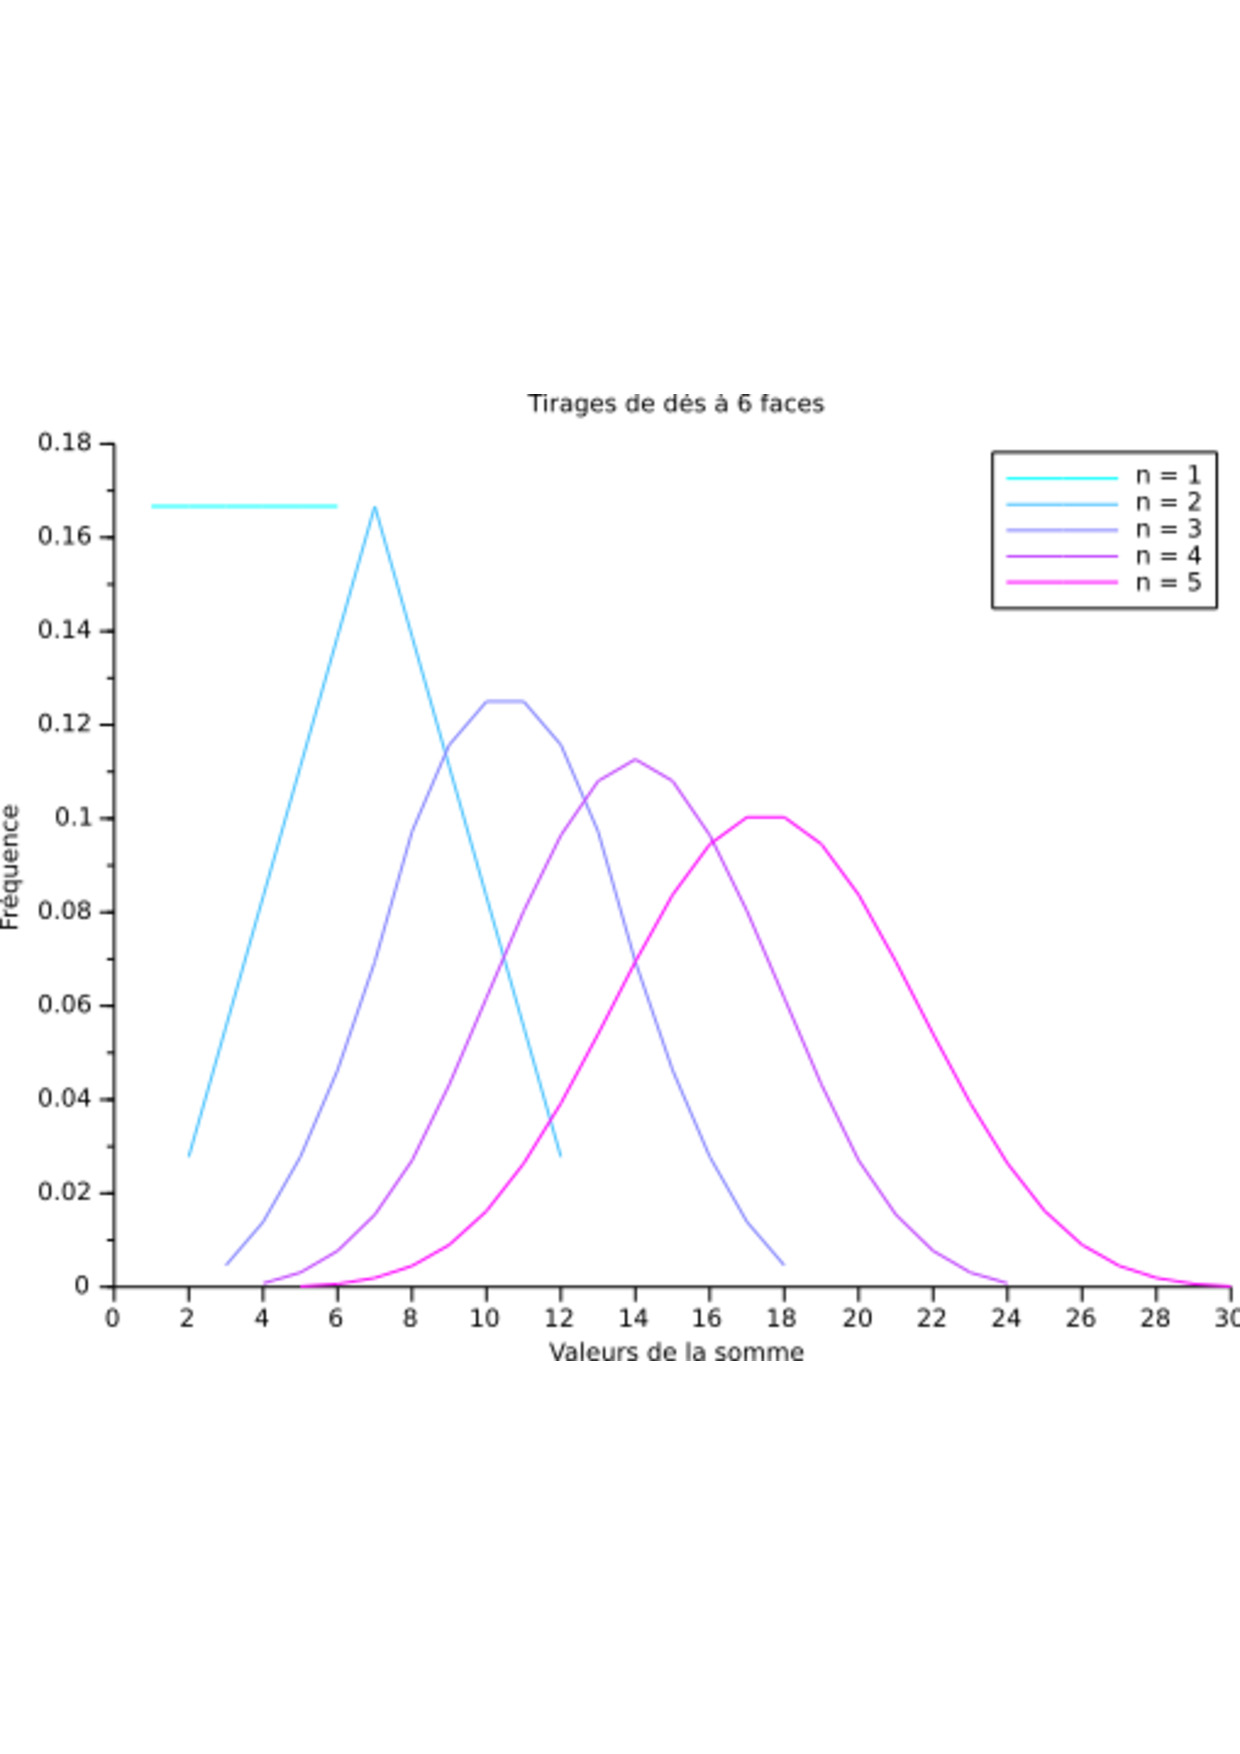
\includegraphics[width=\textwidth,height=0.8\textheight,keepaspectratio]{images/SommeNormale.pdf}
\end{frame}
\begin{frame}{Fonction de densité}
	\pause
	\begin{defn}{}
		La \defi{loi normale de moyenne $\mu$ et de variance $\sigma^2$}, notée $N(\mu,\sigma^2)$, est la loi de probabilité dont la densité est donnée par
		\[f(x)=\frac{1}{\sigma\sqrt{2\pi}}\text{e}^{-\frac{(x-\mu)^2}{2\sigma^2}}.\]
	\end{defn}
Il nous faudra justifier cette appellation en montrant que $\mu$ et $\sigma^2$ correspondent bien à la moyenne et à la variance de la loi.
\begin{lumiere}  Dasn le cas où $\mu=0$ et $\sigma=1$, on dit qu'il s'agit de la \textbf{loi normale standard} ou encore de la \textbf{loi normale centrée et réduite}. La fonction de densité de la loi normale standard est noté $\varphi$ est sa fonction de répartition $\Phi$.
\end{lumiere}
\end{frame}
\begin{frame}{Propriétés}
	\pause
	\begin{prop}
		Si $X\sim N(\mu,\sigma^2)$, alors la variable aléatoire définie par $Z=\frac{X-\mu}{\sigma}$ suit la loi normale standard.
	\end{prop}
	\begin{prop}
		Si $X\sim N(\mu,\sigma^2)$, alors
		\[\P{a<X\leq b}=\Phi\left(\frac{b-\mu}{\sigma}\right)-\Phi\left(\frac{a-\mu}{\sigma}\right).\]
	\end{prop}

\end{frame}
\begin{frame}{Fonction génératrice}
	\pause
	\begin{thm}
		La fonction génératrice des moments de la loi normale de moyenne $\mu$ et de variance $\sigma^2$ est donnée par
		\[M(t)=\exp\left(\mu t+\frac{\sigma^2t^2}{2}\right)\]
	\end{thm}
	La fonction génératrice des moments peut être utilisée pour démontrer le théorème de l'acétate suivante.
\end{frame}
\begin{frame}{Propriétés de la loi normale}
	\pause
	\begin{thm}
		\begin{enumerate}
			\item La moyenne de la loi $N(\mu,\sigma^2)$ est $\mu$;\\
			\item La variance de la loi $N(\mu,\sigma^2)$ est $\sigma^2$;\\
			\item Si $X\sim N(\mu,\sigma^2)$, alors $aX+b\sim N(a\mu+b,a^2\sigma^2)\forall a\in\Rs,b\in\R$;\\
			\item Si $X$ et $Y$ sont deux v.a. indépendantes vérifiant $X\sim N(\mu_X,\sigma_X^2)$ et $Y\sim N(\mu_Y,\sigma_Y^2)$, alors
			\[X+Y\sim N(\mu_X+\mu_Y,\sigma_X^2+\sigma_Y^2).\]
		\end{enumerate}
	\end{thm}
\end{frame}
\begin{frame}{Approximation d'une binomiale par une normale}
	\pause
	\begin{thm}
		Supposons que $X\sim\loibinomiale{n}{p}$ où $np\geq 5, n(1-p)\geq 5$. Supposons que $Y\sim \loinormale{np}{np(1-p)}$. Alors $X\approx Y$.
	\end{thm}

\begin{center}
	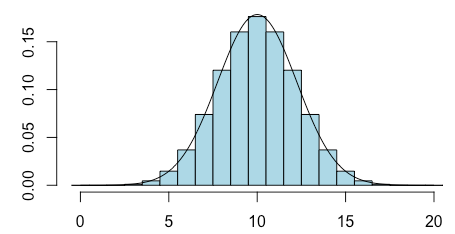
\includegraphics[width=0.55\textwidth]{images/binomok.png}
	{\footnotesize Source : \cite{NormalApproxToBinomial}}
\end{center}
\end{frame}
\begin{frame}[t]{Exemples d'utilisation}
	On lance un dés 100 fois. Quelle est la probabilité d'obtenir un nombre de 3 entre 10 et 20 inclusivement?
\end{frame}
\begin{frame}{Les conditions sur $n$ et $p$}
	\pause
	On exige que $np\geq 5$ et $n(1-p)\geq 5$ pour éviter ces scénarios :
	\begin{center}
		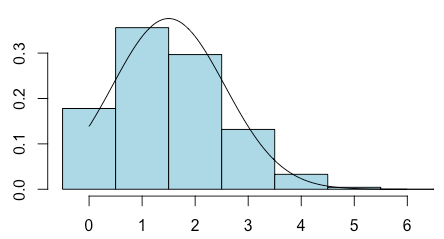
\includegraphics[width=0.5\textwidth]{images/binompasok.png}\hfill 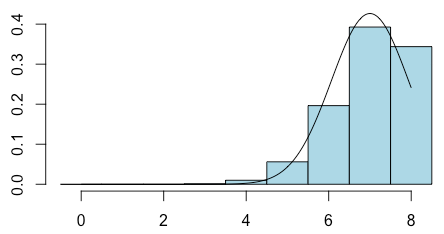
\includegraphics[width=0.5\textwidth]{images/binompasok2.png}\\
		{\footnotesize Source : \cite{NormalApproxToBinomial}}
	\end{center}
\end{frame}
\section{La fonction gamma}
\begin{frame}{Définition et propriétés élémentaires}
La fonction gamma apparaît naturellement dans plusieurs branches des mathématiques (et en physique). Voici la définition que nous considérerons dans le cadre du cours de probabilités.

\begin{defn}{}
	Soit $\alpha\in\intoo{0}{\infty}$. La \defi{fonction gamma} (de Euler) est définie par
	\[\Gamma(\alpha)=\int_{0}^{\infty}t^{\alpha -1}\eu^{-t}\,\dl{t}.\]
\end{defn}
\end{frame}
\begin{frame}{Lien avec la factorielle d'un nombre naturel}
En intégrant par partie, on montre que pour $\alpha>1$,
\[\Gamma(\alpha)=(\alpha-1)\Gamma(\alpha-1).\]
De par cette propriété, on peut voir la fonction gamma comme un prolongement de la fonction factoriel (définie sur les naturels) avec un décalage. Alors que $5!=120$, $\Gamma(5)=4!=24$.
\end{frame}
\begin{frame}{Lien avec la théorie des nombres (facultatif)}
En théorie des nombres, on définit la fonction $\Gamma$ sur $\mathbb{C}~\backslash~\{0,-1,-2,\ldots\}$ par prolongement analytique. Elle est alors reliée à la fonction zêta de Riemann de la manière suivante:
\begin{align*}
\zeta(s) &=\sum_{n=1}^\infty \frac{1}{n^s} =\frac{1}{1^s} + \frac{1}{2^s} + \frac{1}{3^s} + \cdots,\\
\zeta(s) &= 2^s\pi^{s-1} \sin\left(\frac{\pi s}{2}\right) \Gamma(1-s)\zeta(1-s).
\end{align*}
\end{frame}
\section{La loi gamma}
\begin{frame}{La loi gamma}
	\begin{defn}{}
		Soit $\alpha$ et $\lambda$ des éléments de $\intoo{0}{\infty}$. La \defi{loi gamma} de paramètres $\alpha$ et $\lambda$ possède une densité donnée par
		\[f(t)=\begin{cases}
			\frac{\lambda^{\alpha}}{\Gamma(\alpha)}t^{\alpha-1}\eu^{-\lambda t} &\text{si $t>0$,}\\
			0 & \text{sinon.}
		\end{cases}\]
	\end{defn}
Si $X$ suit une loi gamma de paramètres $\alpha$ et $\lambda$, on écrira que $X\sim \Gamma\,(\alpha,\lambda)$. On vérifie aussi qu'en posant $\alpha=1$ dans la fonction de densité de la loi gamma, nous obtenons la fonction de densité d'une exponentielle de paramètre $\lambda$. Ainsi,
\[\Gamma\,(1,\lambda)=\text{exponentielle}\,(\lambda).\]
\end{frame}
\begin{frame}[t]{Lien entre loi gamma et loi exponentielle}
	\begin{thm}
		Supposons que $X_1,X_2,\ldots,X_n$ sont des variables aléatoires i.i.d. qui suivent une loi exponentielle de paramètre $\lambda$. Posons $S=\sum_{k=1}^nX_k$. Alors
		\[S\sim \loigamma{n}{\lambda}.\]
	\end{thm}
\end{frame}
\begin{frame}{Fonction génératrice associée à une distribution gamma}
	\begin{thm}
		La fonction génératrice des moments d'une v.a. de loi $\loigamma{\alpha}{\lambda}$ est donnée par
		\[M(t)=\begin{cases}
			\left(\frac{\lambda}{\lambda -t}\right)^{\alpha}&\text{si $t<\lambda$},\\
			\infty & \text{si $t\geq\lambda$}.\\
		\end{cases}\]
	\end{thm}
	\end{frame}
	\begin{frame}{Propriétés de la distribution gamma}
	\begin{thm}
		Supposons que $X_1,X_2,\ldots,X_n$ sont des variables aléatoires indépendantes telles que $X_k\sim \loigamma{\alpha_k}{\lambda}~\forall k\in\{1,2,\ldots, n\}$. Posons $\xi=\sum_{k=1}^n\alpha_k$ et $S=\sum_{k=1}^nX_k$. Alors
		\[S\sim \loigamma{\xi}{\lambda}.\]
	\end{thm}
	La loi gamma est souvent utilisée pour modéliser des temps d'attente ou des durées.
\end{frame}
\section{La loi de Cauchy}
\begin{frame}[t]{Le problème de l'archer aveugle}
\end{frame}
\begin{frame}[t]{Une distribution sans espérance}
\end{frame}
\begin{frame}[t]{Une simulation}
	\begin{center}
		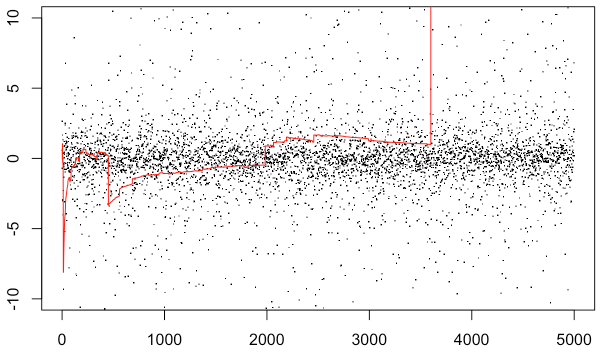
\includegraphics[width=\textwidth,height=0.72\textheight,keepaspectratio]{images/Cauchy1.png}\\
		{\footnotesize Source : \cite{Rickert2017}}
	\end{center}
\end{frame}
\begin{frame}[t]{Un pas derrière}
		\begin{center}
		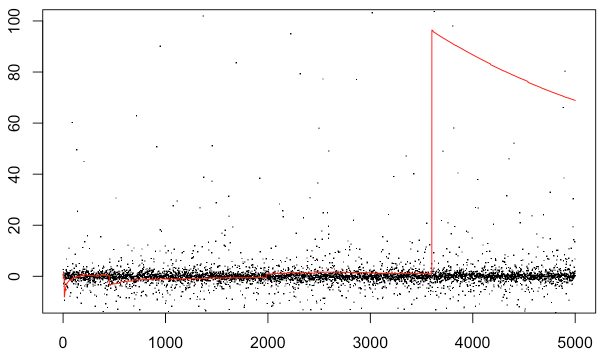
\includegraphics[width=\textwidth,height=0.72\textheight,keepaspectratio]{images/Cauchy2.png}\\
		{\footnotesize Source : \cite{Rickert2017}}
	\end{center}
\end{frame}
\begin{frame}[t]{La queue d'une distribution}
		\begin{center}
		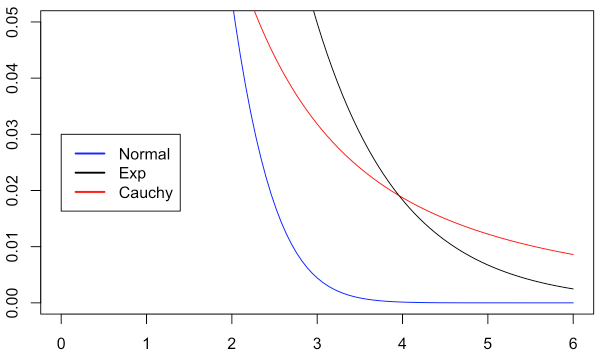
\includegraphics[width=\textwidth,height=0.72\textheight,keepaspectratio]{images/queue.png}\\
		{\footnotesize Source : \cite{Rickert2017}}
	\end{center}
\end{frame}
\begin{frame}[t]{Applications de la loi de Cauchy}
	\begin{thm}
		Soit $X$ et $Y$ des v.a. i.i.d. de loi $\loinormale{0}{1}$. Posons $Z=X/Y$. Alors
		\[Z\sim\loiCauchy{0}{1}.\]
	\end{thm}
	La loi de Cauchy est aussi un cas particulier d'une distribution de Student avec un degré de liberté.
\end{frame}
\begin{frame}[allowframebreaks]{Bibliographie}
\printbibliography[heading=none]
\vspace{0.5cm}

 \begin{rems}
 	\begin{itemize}
 		\item Ce document est rédigé avec Beamer, une classe de \LaTeX.
		\item La formulation des définitions et énoncés est fortement inspirée de \cite{belisle}.
 	\end{itemize}
 \end{rems}

 	\vfill
 	\footnotesize Pour signaler une erreur dans ce document, veuillez écrire à~\href{mailto:jerome.soucy@mat.ulaval.ca}{jerome.soucy@mat.ulaval.ca}.
 \end{frame}
\end{document}